\documentclass{article}
\usepackage{graphicx}
\usepackage{amsmath}
\usepackage{float}
\usepackage{amsthm}
\usepackage{fancyhdr}
\usepackage[breaklinks]{hyperref}
\usepackage[margin=1in]{geometry}
\usepackage{listings}
\usepackage{xcolor}
\usepackage{fontspec}

\newfontfamily\jetbrainsmono{JetBrains Mono}
\definecolor{codebg}{RGB}{255, 245, 255}

\pagestyle{fancy}
\fancyhf{}
\fancyhead[L]{Jeevan Shah \\ RFR Precharge Design}
\fancyhead[R]{\thepage}

\lstdefinelanguage{Zig}{
    keywords={
        const, var, fn, pub, return, if, else, while, for,
        switch, struct, enum, union, error, defer, errdefer,
        try, catch, unreachable, comptime, inline, asm,
        break, continue, and, or, null, undefined, true, false
    },
    keywordstyle=\color{blue}\bfseries,
    comment=[l]{//},
    morecomment=[s]{/*}{*/},
    commentstyle=\color{gray},
    string=[b]",
    stringstyle=\color{red},
    basicstyle=\ttfamily\small,
    numbers=left,
    numberstyle=\tiny\color{gray},
    numbersep=8pt,
    frame=single,
    breaklines=true,
    showstringspaces=false,
    basicstyle=\jetbrainsmono\small,
}

\hypersetup{
    colorlinks=true,
    linktoc=section,
    linkcolor=blue,
}

\title{2027 Digital Precharge}
\author{Jeevan Shah}


\begin{document}
\begin{titlepage}
	\centering
	\vfill

	{\Huge \textbf{Precharge Design Report}\par}

	\vspace{0.5cm}

	{\Large Rutgers Formula Racing\par}

	\vspace{0.5cm}

	{\large Jeevan Shah \par}
	{\large \today \par}

	\vspace{2.5cm}

	
\includegraphics[width=0.5\textwidth]{RFR EV Logo White Bolt - Black Letters - Red Body.png}

	\vfill
\end{titlepage}

\newpage

\tableofcontents

\newpage

\section{Revision Log}
\begin{tabular}{| c | c | c |}
	\hline
	Editor      & Date         & Revision \\
	\hline
	Jeevan Shah & Aug. 12 2026 & 1        \\
	\hline
\end{tabular}

\section{Purpose}
Investigate and plan the switch to a microcontroller based precharge system for the 2027 FSAE season.

\section{Parties Involved}
\begin{tabular}{| c | c | c |}
	\hline
	Name        & Team Role                            & Report Role \\
	\hline
	Jeevan Shah & Electronics co-Lead \& Software Lead & Author      \\
	\hline
\end{tabular}

\section{Research}
\subsection{Relevant Rules}
\begin{enumerate}
	\item[\textbullet] \textbf{EV.5.6.1} The Accumulator must contain a Precharge Circuit. The Precharge Circuit must:
	      \begin{enumerate}
		      \item Be able to charge the Intermediate Circuit to minimum 90\% of the Accumulator voltage before closing the second IR.
		      \item Be supplied from the Shutdown Circuit EV.7.1.
	      \end{enumerate}

	\item[\textbullet] \textbf{EV.5.6.2} The Intermediate Circuit must precharge before closing the second IR.
	      \begin{enumerate}
		      \item The end of precharging must be controlled by feedback by monitoring the voltage in the Intermediate Circuit.
	      \end{enumerate}

	\item[\textbullet] \textbf{EV.5.6.3} The Tractive System must contain a Discharge Circuit. The Discharge Circuit must be:
	      \begin{enumerate}
		      \item Wired in a way that it is always active when the Shutdown Circuit is open.
		      \item Able to discharge the Intermediate Circuit capacitors if the MSD has been opened.
		      \item Not be fused.
		      \item Designed to handle the maximum Tractive System voltage for minimum 15 seconds.
	      \end{enumerate}

	\item[\textbullet] \textbf{EV.5.6.4} Positive Temperature Coefficient (PTC) devices must not be used to limit current for the Precharge Circuit or Discharge Circuit.

	\item[\textbullet] \textbf{EV.5.6.5} The precharge relay must be a mechanical type relay.

	\item[\textbullet] \textbf{EV.6.5.7} Voltage Separation
	      \begin{enumerate}
		      \item HV and GLV must be separated galvanically. If on same board, spacing requirements must be met.
	      \end{enumerate}
\end{enumerate}

\subsection{Why Do We Need This?}
The RFR '26 season came to end when E-meter data was pulled during EV-active revealing that our precharge was not functional and instead closing both isolation relays (IRs) at the same time. Extensive testing and debugging of both RFR '26's and RFR 25's precharge board revealed that there seemed to be a fundatmental issue in our design as when both board were supplied with high voltages and high capacitance (i.e. tested in the car), both IRs still shut instantly. Switching to a microcontroller based system allows us to read both the inverter and battery management system (BMS) voltages via CAN which, when coupled with basic software logic, helps ensure that the IRs will never close early.

\subsection{Pros \& Cons}
\begin{minipage}[t]{0.45\linewidth}
	\begin{center}
		\textbf{Pros}
		\begin{enumerate}
			\item A microcontroller based system is very easy to change and modify compared to an analog system
			\item Using software logic to regulate the IRs ensures that they will never close early
			\item The microcontroller implementation iterates off of RFR '26's precharge design, keeping the high voltage section which has been proven to work
		\end{enumerate}
	\end{center}
\end{minipage}
\hfill
\begin{minipage}[t]{0.45\linewidth}
	\begin{center}
		\textbf{Cons}
		\begin{enumerate}
			\item Team members must know how to code and work with embedded systems to work and troubleshoot
			\item Changing our precharge design may result in difficulties involved with passing ESF
		\end{enumerate}
	\end{center}
\end{minipage}

\subsection{Design Impact}
The size of the PCB will not change, which means currently implemented packaging solutions will hold valid for the RFR '27 season. Any weight changes are non-negligible due to the an about equivalent amount of components swapped from the previous design.

\section{Notes/Finding}
\subsection{Core Requirements}
The core functionality of the precharge circuit is
\begin{enumerate}
	\item to be powered off of the shutdown circuit (SDC)
	\item close the first IR as soon as the SDC is closed
	\item close the second IR once the inverter voltage is (at least) 90\% of the total BMS voltage at any given state of charge (SOC)
	      \begin{enumerate}
		      \item it follows that the precharge must monitor the BMS and inverter voltage
	      \end{enumerate}
\end{enumerate}

\subsection{Part Choices and Justification}
Because we are iterating on a previous design it is known that our precharge will function off of 24V from the shutdown circuit (SDC). The SHV24-1A85-78D3K reed relay from Standex-Meder electronics will be reused as it is proven to work in two other designs and past EVs, has previously been granted ESF approval, and has a reasonably low 288mW power consumption. We will also utilize the STM32F103T8U6 microcontroller from ST electronics since the STM32F series was utilized in RFR '26 with the sucessful implementation of a custom thermistor module. The STM32F103T8U6 was choosen in specific because it is the most basic microcontroller from ST that has CAN communication capabilities. A more advanced/powerful microcontroller is not needed as the software, general purpose input and output pin (GPIO), and memory requirement are extremely low. The STM32F103T8U6 requires 3.3V as input, which is notably lower than 24V. Because of this, we will utilize the IMA0124S3V3 DCDC converter from XP Power to bring our 24V supply voltage down to 3.3V. The IMA0124S3V3 will also power the non-isolated Texas Instruments CANTransciever TCAN3413DR, enabling us to read CAN frames from both the inverter and BMS.

\subsection{Schematic}
\begin{figure}[H]
	\centering
	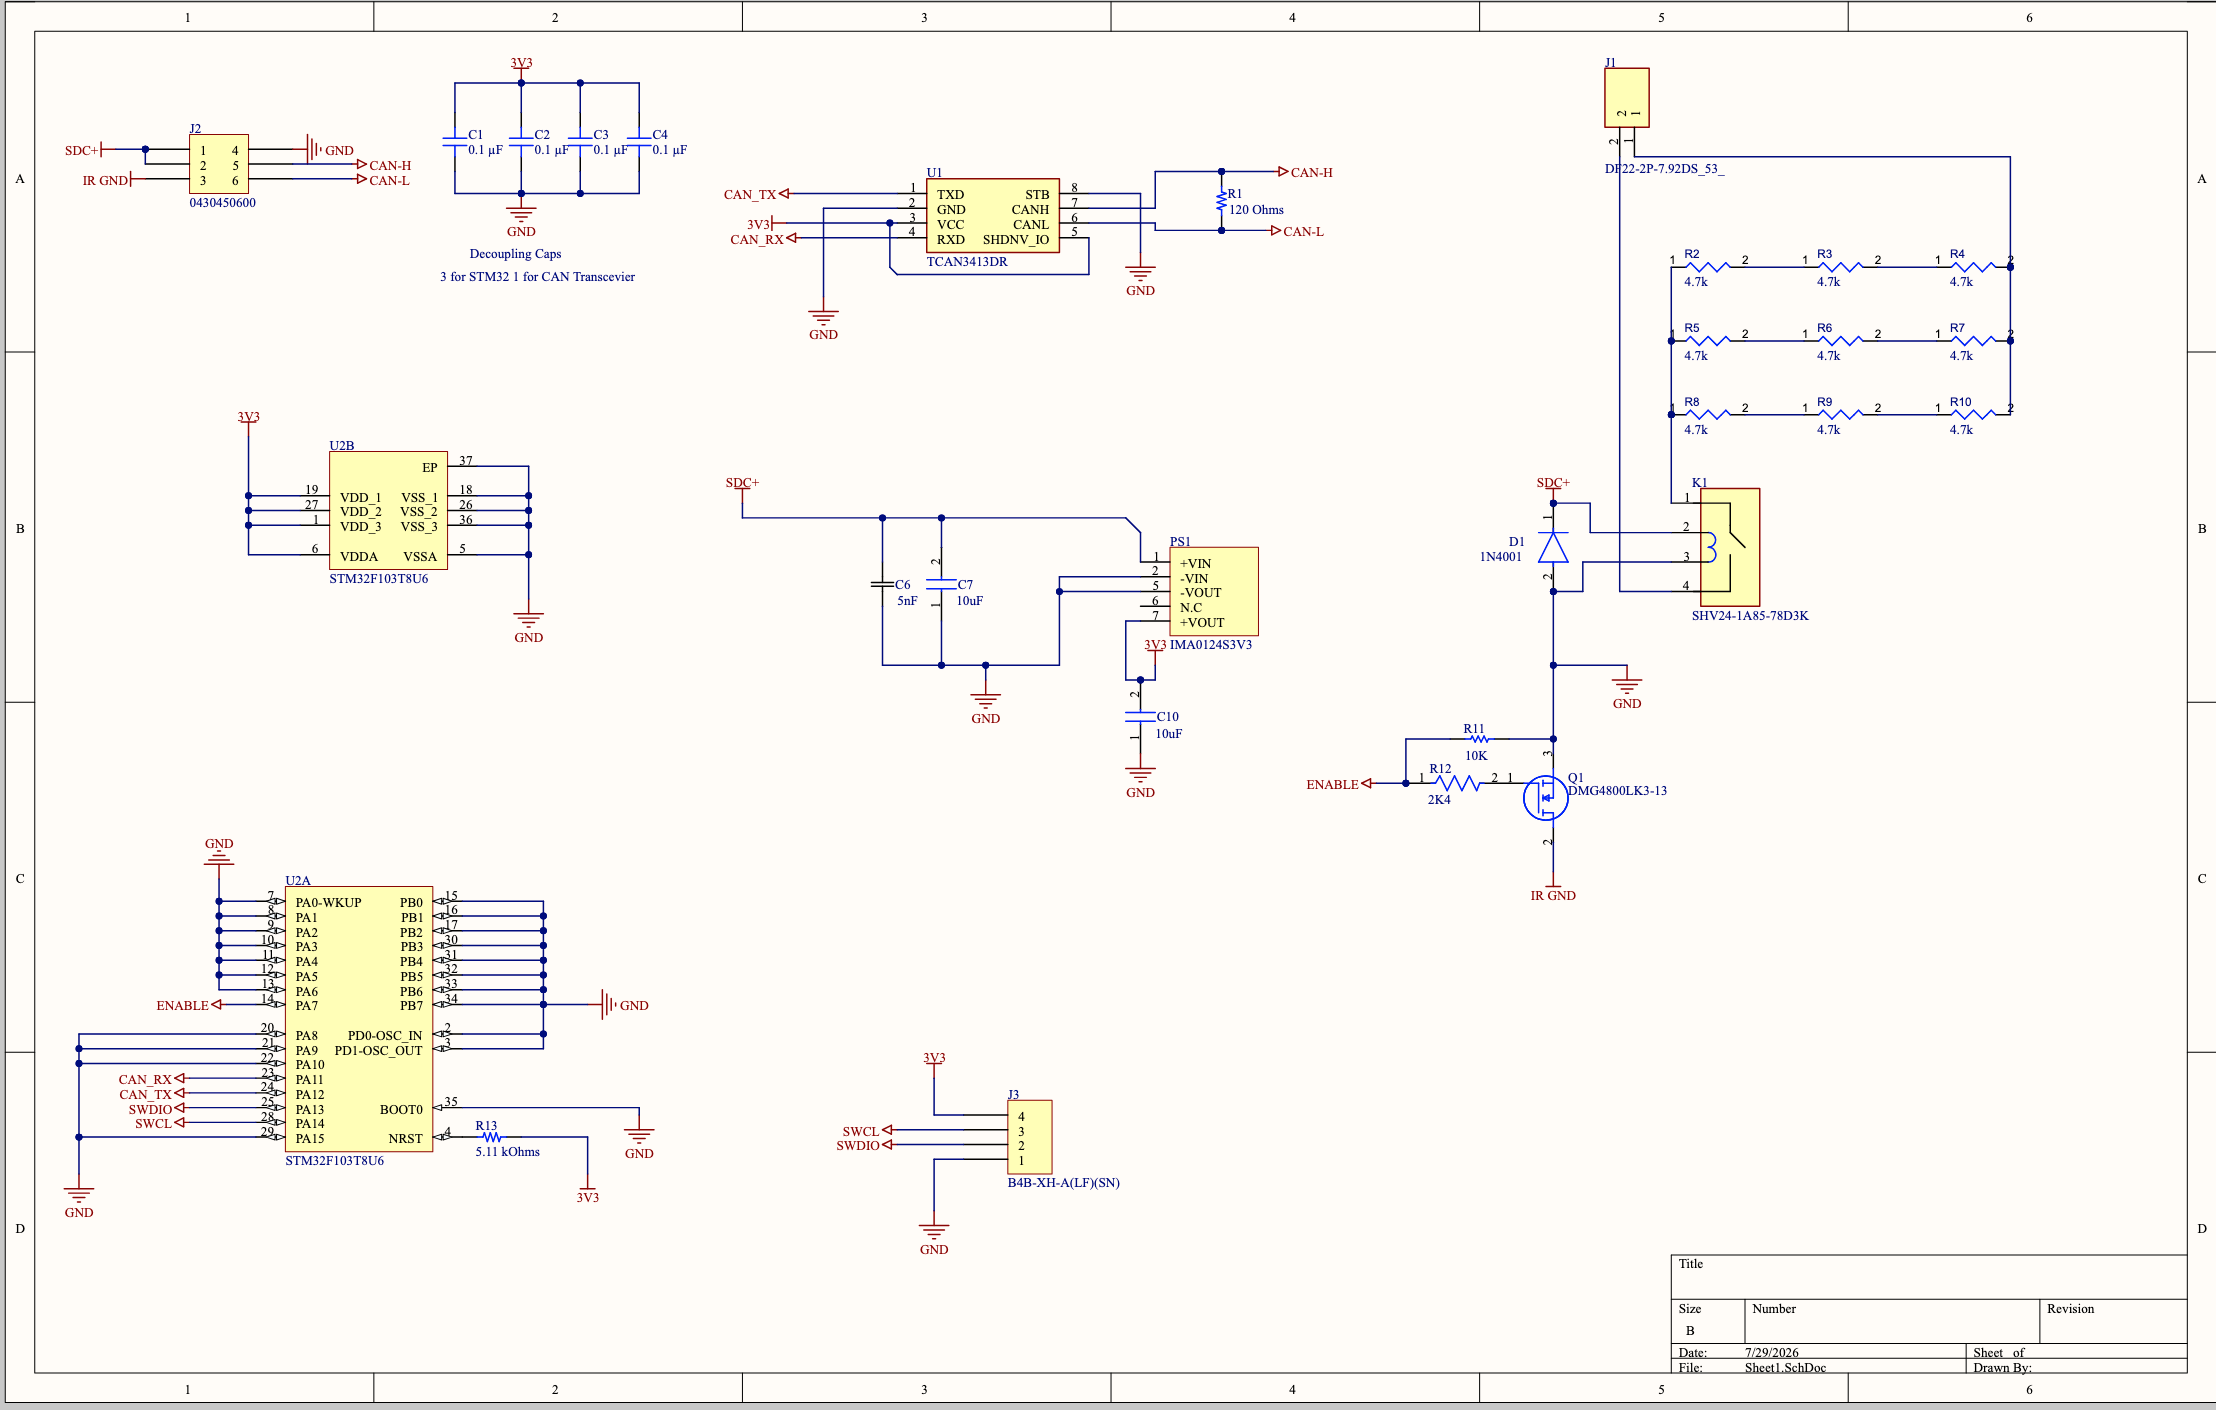
\includegraphics[width=\linewidth]{schematic.png}
	\caption{Schematic}
	\label{fig:schematic}
\end{figure}

The schematic is extremely simple as it only features the microcontroller, DCDC converter, CANTransciever, and the high voltage relay. We are taking advantage of a GPIO pin (labeled `ENABLE') to switch the MOSFET. As mentioned earlier the IMA0124S3V3 is used to convert the 24V SDC supply into a usable 3.3V for the microcontroller and CANTransciever. The relay section (A5, B5) remains mostly identical from the previous design, save for the fact that the third input is no longer needed as voltages are no longer being scaled. The current draw of the STM32 along with the CANTransciever combined is about 110mA, even with the additional decoupling capacitors the 300mA rating of the DCDC converter should never be exceeded.

\subsection{Firmware}
The embedded code that run on the microcontroller is written in \texttt{Zig} - a low level language that works as an alternative to \texttt{C} while providing no hidden overloads. This is a major benefit to working in \texttt{Zig} as the code you read is exactly what is happening. Structually, the code is split into two files: \texttt{main.zig} and \texttt{root.zig}. \texttt{root.zig} serves as the abstract class definitions while \texttt{main.zig} contains the actual implementation as per our setup. For interfacing with the STM32, we utilized the \texttt{microzig} library.

\subsubsection{\texttt{main.zig}}
The \texttt{main.zig} file is extremely simple. Starting at the top, there are the basic imports and setup functions.

\begin{lstlisting}[language=Zig]
const std = @import("std");
const microzig = @import("microzig");
const logic = @import("root.zig");
const stm32 = microzig.hal;
const peripherals = microzig.chip.peripherals;
const rcc = stm32.rcc;
const gpio = stm32.gpio;
const time = stm32.time;

pub const microzig_options: microzig.Options = .{ .interrupts = .{} };
pub const panic = microzig.panic;
pub const std_options = microzig.std_options(.{});

comptime {
    _ = microzig.export_startup();
}

const protocol = logic.base_config;
const loop_period_ms: u32 = 5;

const pins = struct {
    const enable = gpio.Pin.from_port(.A, 7);
    const can_rx = gpio.Pin.from_port(.A, 11);
    const can_tx = gpio.Pin.from_port(.A, 12);
};

fn systemClockConfig() !void {
    _ = try rcc.apply(.{
        .SYSCLKSource = .PLL1_P,
        .PLLSourceVirtual = .HSE_Div_PREDIV,
        .PLLMUL = .Mul9,
        .AHBCLKDivider = .Div1,
        .APB1CLKDivider = .Div2,
        .ADCPresc = .Div6,
        .flags = .{ .HSEOscillator = true },
    });
}
\end{lstlisting}

Following the imports and setup comes the CAN configuration for the STM32. The \texttt{packedFilterID()} function converts a logical CAN ID into the bit layout required by the STM32 bxCAN acceptance-filter registers. This is then used on lines \texttt{69} and \texttt{70} to configure \texttt{FIFO0} (the CAN mailbox queue) to only allow the BMS and inverter CAN frames to be read.

\begin{lstlisting}[language=Zig, firstnumber=38]
fn packedFilterId(spec: logic.VoltageSpec) u32 {
    return switch (spec.kind) {
        .extended => ((spec.id & 0x1FFF_FFFF) << 3) | (1 << 2),
        .standard => (spec.id & 0x7FF) << 21,
    };
}

fn canInit() void {
    const can = peripherals.CAN;

    // Enter initialization mode before changing bit timing.
    can.MCR.modify(.{ .SLEEP = 0, .INRQ = 1 });
    while (can.MSR.read().INAK == 0) {}

    // APB1 is 36 MHz. BRP=4, 18 time quanta/bit gives 500 kbit/s;
    // register fields contain each value minus one.
    if (protocol.bitrate != 500_000)
        @compileError("Update bxCAN bit timing before selecting another bitrate");
    can.BTR.modify(.{
        .BRP = 3,
        .@"TS[0]" = 14,
        .@"TS[1]" = 1,
        .SJW = 0,
        .LBKM = 0,
        .SILM = .Normal,
    });

    can.FMR.modify(.{ .FINIT = 1 });
    can.FM1R.raw |= 1; // bank 0, identifier-list mode
    can.FS1R.raw |= 1; // bank 0, 32-bit scale
    can.FFA1R.raw &= ~@as(u32, 1); // bank 0 -> FIFO0
    can.FB[0].FR1.raw = packedFilterId(protocol.bms);
    can.FB[0].FR2.raw = packedFilterId(protocol.inverter);
    can.FA1R.raw |= 1;
    can.FMR.modify(.{ .FINIT = 0 });

    can.MCR.modify(.{ .INRQ = 0 });
    while (can.MSR.read().INAK == 1) {}
}

fn canReceive() ?logic.Frame {
    const can = peripherals.CAN;
    if (can.RFR[0].read().FMP == 0) return null;

    const fifo = &can.RX[0];
    const rir = fifo.RIR.read();
    var frame = logic.Frame{
        .id = undefined,
        .kind = if (rir.IDE == .Extended) .extended else .standard,
        .remote = rir.RTR == .Remote,
        .dlc = fifo.RDTR.read().DLC,
        .data = undefined,
    };
    frame.id = switch (frame.kind) {
        .extended => (@as(u32, rir.STID) << 18) | rir.EXID,
        .standard => rir.STID,
    };
    std.mem.writeInt(u32, frame.data[0..4], fifo.RDLR.raw, .little);
    std.mem.writeInt(u32, frame.data[4..8], fifo.RDHR.raw, .little);

    can.RFR[0].modify(.{ .RFOM = 1 });
    return frame;
}
\end{lstlisting}

Following the CAN setup is the \texttt{main()} function which contains the master superloop for the program. The first ten lines contain the clock setup, pin setup, and initalization of the timer variable and the primary controller.

\begin{lstlisting}[language=Zig, firstnumber=101]
pub fn main() !void {
    try systemClockConfig();

    rcc.enable_clock(.GPIOA);
    rcc.enable_clock(.AFIO);
    rcc.enable_clock(.CAN);
    rcc.enable_clock(.TIM2);

    // Establish the safe output state before initializing communications.
    pins.enable.put(0);
    pins.enable.set_output_mode(.general_purpose_push_pull, .max_2MHz);
    pins.can_rx.set_input_mode(.floating);
    pins.can_tx.set_output_mode(.alternate_function_push_pull, .max_50MHz);

    time.init_timer(.TIM2);
    canInit();

    var now_ms: u32 = 0;
    var controller = logic.Controller.init(protocol, now_ms);
\end{lstlisting}

Entering into the primary superloop, there are four main sections. Lines $120-121$ contains the entry to the superloop and unpacks CAN frames.
\begin{lstlisting}[language=Zig, firstnumber=120]
    while (true) {
       while (canReceive()) |frame| controller.ingest(frame, now_ms);
\end{lstlisting}

Next, the \texttt{tick()} function is called which updates the \texttt{state} variable.
\begin{lstlisting}[language=Zig, firstnumber=122]
        controller.tick(now_ms);
\end{lstlisting}

Then, the program checks the updated state. If precharging is complete, then the enable pin is set to high, and an infinite loop is entered. If there was a fault, then the enable pin stays low and an infinite loop is entered. In any of the other states (\texttt{waiting\_for\_bms} or \texttt{precharging}) no further action is taken.
\begin{lstlisting}[language=Zig, firstnumber=last]
        switch (controller.state) {
            .complete => {
                pins.enable.put(1);
                while (true) time.sleep_ms(1_000);
            },
            .fault_latched => {
                pins.enable.put(0);
                while (true) time.sleep_ms(1_000);
            },
            else => {},
       }
\end{lstlisting}

Finally, there is a brief delay before the next cycle is entered to ensure that there is necessary time for the CAN mailbox to be flushed, and the timer variable \texttt{now\_ms} is updated.
\begin{lstlisting}[language=Zig, firstnumber=last]
        time.sleep_ms(loop_period_ms);
        now_ms +%= loop_period_ms; // leverage wrapping addition to keep the timer going 
    }
}
\end{lstlisting}

\subsubsection{\texttt{root.zig}}
As mentioned earlier, \texttt{root.zig} contains the abstract \texttt{Controller} class which is used in \texttt{main.zig}. Within \texttt{root.zig} are multiple enum and const definitions, but for the purpose of this document I will simply be reviewing the primary functions used.


The \texttt{ingest()} function (see \texttt{main.zig:121}), comes from \texttt{root.zig}. At its core, \texttt{ingest()} reads a CAN frame and decides if it is from the BMS or the inverter. For either source, the program will convert the CAN frame into a voltage-via the \texttt{decodeVoltage()} function-and then the voltage is updated along with the timestamp. If the frame is from the BMS then there is a check to update the state from \texttt{waiting\_for\_bms} to \texttt{precharge} which happens when the first BMS frame is recieved as \texttt{waiting\_for\_bms} is the default state. If the frame is from the inverter then the \texttt{qualify()} function is called.
\begin{lstlisting}[language=Zig, backgroundcolor=\color{codebg}, firstnumber=107]
    pub fn ingest(self: *Controller, frame: Frame, now_ms: u32) void {
        if (self.state == .complete or self.state == .fault_latched) return;

        if (matches(frame, self.config.bms)) {
            const value = decodeVoltage(frame, self.config.bms) catch {
                self.latch(.malformed_frame);
                return;
            };
            if (!self.plausible(value)) return self.latch(.implausible_voltage);
            self.bms = .{ .value = value, .timestamp_ms = now_ms };
            if (self.state == .waiting_for_bms) {
                self.state = .precharging;
                self.precharging_started_ms = now_ms;
            }
        } else if (matches(frame, self.config.inverter)) {
            const value = decodeVoltage(frame, self.config.inverter) catch {
                self.latch(.malformed_frame);
                return;
            };
            if (!self.plausible(value)) return self.latch(.implausible_voltage);
            self.inverter = .{ .value = value, .timestamp_ms = now_ms };
            self.qualify(now_ms);
        }
    }
\end{lstlisting}

The \texttt{qualify()} function is where the actual logic lives to decide whether or not to close the IR. Up to line $165$ is basic setup and fault checking. Lines $155-158$ checks if a BMS voltage exists, and if not it sets the amount of consecutive qualifying samples to $0$ and returns early. Next, lines $160-163$ check to ensure that the most recent BMS voltage reading is less than a defined threshold (\texttt{freshness\_timeout\_ms}), if it isn't, a fault is thrown. Finally, lines $165-173$ check whether the inverter voltage is greater than $90\%$ of the BMS voltage. If it is, the \texttt{consecutive\_qualifying} variable is increased. After \texttt{qualifying\_samples} amount of valid consecutive frames, precharging is complete.
\begin{lstlisting}[language=Zig, backgroundcolor=\color{codebg}, firstnumber=154]
    fn qualify(self: *Controller, now_ms: u32) void {
        const bms = self.bms orelse {
            self.consecutive_qualifying = 0;
            return;
        };
        const inverter = self.inverter.?;
        if (elapsed(now_ms, bms.timestamp_ms) >= self.config.freshness_timeout_ms) {
            self.latch(.stale_data);
            return;
        }

        const lhs = @as(u64, inverter.value) * 100;
        const rhs = @as(u64, bms.value) * self.config.threshold_percent;
        if (lhs >= rhs) {
            self.consecutive_qualifying +|= 1; // saturating addition prevents wrapping to zero
            if (self.consecutive_qualifying >= self.config.qualifying_samples)
                self.state = .complete;
        } else {
            self.consecutive_qualifying = 0;
        }
    }
\end{lstlisting}

The final primary function in \texttt{root.zig} is the \texttt{tick()} function. The \texttt{tick()} function's primary purpose is to ensure that there is no stale data. The function ensures that the entire precharge cycle isn't taking too long (lines $134-135$), the BMS has sent its first frame within \texttt{freshness\_timeout\_ms} (lines $137-141$), the most recent BMS and inverter frames are within \texttt{freshness\_timeout\_ms} (lines $143-148$), and that the time for the inverter voltage to reach $90\%$ of the BMS voltage is within \texttt{freshness\_timeout\_ms}.
\begin{lstlisting}[language=Zig, backgroundcolor=\color{codebg}, firstnumber=132]
    pub fn tick(self: *Controller, now_ms: u32) void {
        if (self.state == .complete or self.state == .fault_latched) return;
        if (elapsed(now_ms, self.started_ms) >= self.config.precharge_timeout_ms)
            return self.latch(.timeout);

        if (self.state == .waiting_for_bms) {
            if (elapsed(now_ms, self.started_ms) >= self.config.freshness_timeout_ms)
                self.latch(.stale_data);
            return;
        }

        const bms = self.bms orelse return self.latch(.stale_data);
        if (elapsed(now_ms, bms.timestamp_ms) >= self.config.freshness_timeout_ms)
            return self.latch(.stale_data);
        if (self.inverter) |reading| {
            if (elapsed(now_ms, reading.timestamp_ms) >= self.config.freshness_timeout_ms)
                return self.latch(.stale_data);
        } else if (elapsed(now_ms, self.precharging_started_ms.?) >= self.config.freshness_timeout_ms) {
            return self.latch(.stale_data);
        }
    }
\end{lstlisting}

The default config can be seen below.
\begin{lstlisting}[language=Zig, backgroundcolor=\color{codebg}]
pub const ProtocolConfig = struct {
    ready: bool,
    bitrate: u32,
    bms: VoltageSpec,
    inverter: VoltageSpec,
    min_voltage: u32 = 1,
    max_voltage: u32 = 390,
    threshold_percent: u8 = 90,
    qualifying_samples: u8 = 1,
    freshness_timeout_ms: u32 = 5_000,
    precharge_timeout_ms: u32 = 300_000,
};
\end{lstlisting}

View the entire codebase on the \href{https://github.com/rutgers-fsae/firmware/tree/main/precharge}{Rutgers Formula Racing Github} for more.

\section{Conclusion}
Switching to a microcontroller based precharge system allows us to implement something that is more reliable and easier to modify than the analog alternative.
\end{document}
